
\section{Data Model for Project, Dataset and User Management}

The data model used for the management of the different files and the authentication system will be explained in this and the following section, respectively.

A relational database for project, dataset and user management was created using the MySQL \gls{rdbms}. The tables that constitute the database are the \textit{user}, \textit{project}, \textit{permission}, \textit{dataset} and \textit{datatype} tables. The MySQL model used in the platform for project, dataset and user management is shown in \autoref{database}.

\begin{figure}[h]
	\centering
	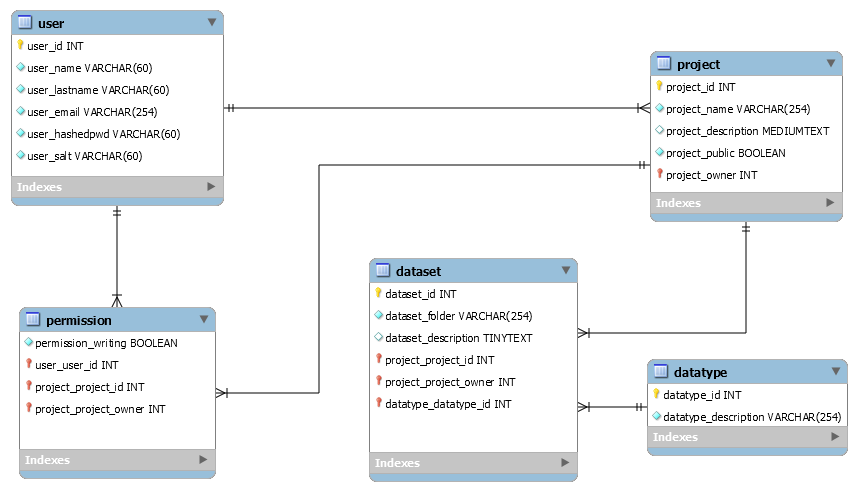
\includegraphics[width=0.95\linewidth]{Imagens/database}
	\caption{MySQL model used in the platform for project, dataset and user management.}
	\label{database}
\end{figure}

The \textit{user} table has a \textit{user\_id} attribute to store each user's unique identifier, a \textit{user\_name} attribute to store the user's first name, a \textit{user\_lastname} attribute to store the user's last name, a \textit{user\_email} attribute to store the user's email, a \textit{user\_hashedpwd} attribute to store the encrypted password and a \textit{user\_salt} attribute which stores the salt associated with the password. The password encryption process will be explained in the next section. 

The \textit{user} table has a 1:N relationship with the \textit{project} table, meaning a user can have one or more projects. \textit{Project} table has a \textit{project\_id} attribute to store each project's identifier, a \textit{project\_name} attribute to store the project's name, a \textit{project\_description} optional attribute to store the project's description, a \textit{project\_public} attribute that stores a boolean value indicating whether or not the project is public and a foreign key \textit{project\_owner} which references to the \textit{user}'s table \textit{user\_id} attribute.

Projects can either be public, and every user has access to them, or private, in which case only the creator has access. These permissions are handled in the \textit{permission} table, which has a \textit{permission\_writing} attribute that stores a Boolean value according to the privacy of a project. Both \textit{user} and \textit{project} tables have a 1:N relationship with the \textit{permission} table. The \textit{user\_user\_id} foreign key references to the \textit{user\_id} attribute in the \textit{user} table, whereas the \textit{project\_project\_id} and \textit{project\_project\_owner} reference to the \textit{project\_id} and \textit{project\_owner} attributes in the \textit{project} table, respectively.

The dataset information is stored in the \textit{dataset} table, which has a \textit{dataset\_id} attribute to store each dataset's unique ID, a \textit{dataset\_folder} attribute to store the dataset name and a \textit{dataset\_description} optional attribute to store the dataset description. Each dataset has an associated data type, which is stored in the \textit{datatype} table. This table has a \textit{datatype\_id} attribute that stores each data type unique ID and a \textit{datatype\_description} attribute to store the data type name. 

Both \textit{datatype} and \textit{project} tables have a 1:N relationship with the \textit{dataset} table. In this table, the \textit{datatype\_datatype\_id} foreign key references to the \textit{datatype\_id} attribute in the \textit{datatype} table, whereas the \textit{project\_project\_id} and \textit{project\_project\_owner} reference to the \textit{project\_id} and \textit{project\_owner} attributes in the \textit{project} table, respectively.

While the management itself is done using the database, the files are stored in the local file system rather than the database, which only stores the paths to the files.


\section{Password Encryption for Authentication System} \label{password}

For the password encryption process the \textit{bcrypt} R package was used (\href{https://CRAN.R-project.org/package=bcrypt}{\nolinkurl{https://CRAN.R-project.org/package=bcrypt}}). It consists in an R  interface to the OpenBSD 'blowfish' password hashing algorithm, as described in \cite{provos1999future}.

Hashing is the transformation of a string of characters into a usually shorter fixed-length value or key that represents the original string. The hashing process is performed by a hash function, whose returned values are often called hash values, hash codes, digests, or simply hashes. This is a one-way function in which a hashed value cannot be reversed to obtain the original input value (i.e. the password). These functions generate random bytes or numbers from OpenSSL (\href{https://www.openssl.org/}{\nolinkurl{https://www.openssl.org/}}). This provides a cryptographically secure alternative to R's default random number generator. 

\textit{Bcrypt} has the option to incorporate a salt, that is, a random data that is used as an additional input to the hash function, providing additional defense against dictionary attacks or against its hashed equivalent, a pre-computed rainbow table attack. \textit{Bcrypt} is an adaptive function: over time, the iteration count can be increased to make it slower, so it remains resistant to brute-force search attacks even with increasing computation power.

For each password chosen by the users a random salt is generated, using the \textit{gensalt} function, which is stored in the database. The password string is then hashed with the generated salt using the \textit{hashph} function, and the hash code stored in the database as well. 

To authenticate a user, when the application receives a username and password, it performs the hashing operation using the password and stored salt and compares the resulting hashed value with the password hash stored in the database for the particular user. If the two hashes are an exact match, the user provided a valid username and password (\autoref{hash}).

\begin{figure}[h]
	\centering
	\includegraphics[width=0.85\linewidth]{Imagens/hash}
	\caption{Graphical representation of the hashing process.}
	\label{hash}
\end{figure}


Below is a simple example of password hashing in R using the \textit{bcrypt} package:


\begin{lstlisting}[language = R]
library(bcrypt)

password = '12345'
salt = gensalt(log_rounds = 12)
salt
## "$2a$12$.RGbTpgZ8TyBpP.MJUFXMu"

hash = hashpw(password, salt)
hash
## "$2a$12$.RGbTpgZ8TyBpP.MJUFXMubcbSTfHve1cnkHohULAIoDLWq580pNG"

identical(hash, hashpw(password, salt))
## TRUE

\end{lstlisting}

The prefix "\$2a\$12\$" in the hash string specifies a cost parameter of 12, indicating $2^{12}$ key expansion rounds. The random generated salt is ".RGbTpgZ8TyBpP.MJUFXMu" and the resulting hash for the "12345" password is ".RGbTpgZ8TyBpP.MJUFXMubcbSTfHve1cnkHoh-ULAIoDLWq580pNG". These are the values that would be stored in the database, rather than the password itself.

